%%%%%%%%%%%%%%%%%%%%%%%%%%%%%% -*- Mode: Latex -*- %%%%%%%%%%%%%%%%%%%%%%%%%%%%
%%% al_eval.tex --- 
%%% Author          : blehr
%%% Created On      : Sun Mar 28 02:28:57 1993
%%% Last Modified By: blehr
%%% Last Modified On: Sun Apr 11 14:56:40 1993
%%% RCS revision    : $Revision: 1.8 $ $Locker:  $
%%% Status          : In writing....
%%%%%%%%%%%%%%%%%%%%%%%%%%%%%%%%%%%%%%%%%%%%%%%%%%%%%%%%%%%%%%%%%%%%%%%%%%%%%%

\section{Evaluation}
\label{algo:eval}

In this section, the {\octopus} eye-tracking algorithm described in
the previous sections is evaluated with respect to the algorithmic
problem definition given in Section~\ref{intro:problem}.  First, the
overall number of operations for the algorithm is derived in
Section~\ref{algo:eval:O}.  In Section~\ref{algo:eval:test}, an
implementation (previously referred to as the {\em current\/}
implementation) is run on the set of test images presented in
Fig.~\ref{fig:testimages} and the results returned are discussed with
respect to both accuracy and time consumption.  Lastly in
Section~\ref{algo:eval:improve}, some suggestions as to how to improve
the performance and accuracy of the algorithm are presented.

\subsection{Overall Number of Operations}
\label{algo:eval:O}

In Section~\ref{algo:seek:O}, it was shown that the swimming octopus
search algorithm, described in Section~\ref{algo:seek} and
implementing Step 1 of the basic algorithm formulation, performs in
$O(N)$ time when applied to an $N\times N$ image.  In
Section~\ref{algo:pos:O} it was shown that the position determining
algorithm described in Section~\ref{algo:pos}, implementing Step 2 of
the basic algorithm formulation, performs in $O(N)$ time.  Thus it can
be concluded that the {\octopus} eye-tracking algorithm, being
composed of the given implementations of Steps 1 and 2 of the basic
algorithm formulation, performs in $O(N)$ time.  Taking into account
that the number of locations in the image at which the edge detection
operators of Fig.~\ref{fig:masks} have to employed, assuming
relatively good image quality, is $O(1)$ (cf.\ 
Section~\ref{algo:pos:O}), the advantage of {\octopus} over a
``traditional'' approach in terms of computational cost is evident.

\subsection{Test Results}
\label{algo:eval:test}

\begin{figure}[tb]
  \paragraph{}
  \makebox[0.425\textwidth][r]{
    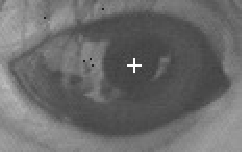
\includegraphics[width=0.3\textwidth]{figurer/posbl01.pdf}}
  \makebox[0.45\textwidth][l]{
    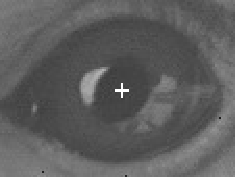
\includegraphics[width=0.3\textwidth]{figurer/posbr01.pdf}}
  \hspace*{0.28\textwidth}(a)\hspace*{0.38\textwidth}(b)
  \paragraph{}
  \makebox[0.425\textwidth][r]{
    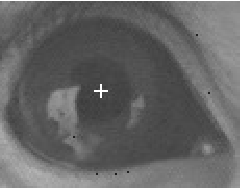
\includegraphics[width=0.3\textwidth]{figurer/posbl02.pdf}}
  \makebox[0.45\textwidth][l]{
    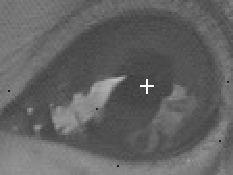
\includegraphics[width=0.3\textwidth]{figurer/posbr02.pdf}}
  \hspace*{0.28\textwidth}(c)\hspace*{0.38\textwidth}(d)
  \paragraph{}
  \makebox[0.425\textwidth][r]{
    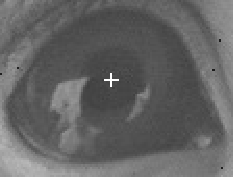
\includegraphics[width=0.3\textwidth]{figurer/posbl05.pdf}}
  \makebox[0.45\textwidth][l]{
    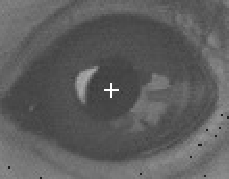
\includegraphics[width=0.3\textwidth]{figurer/posbr03.pdf}}
  \hspace*{0.28\textwidth}(e)\hspace*{0.38\textwidth}(f)
  \caption{\label{fig:results}Returned estimates of the pupil position
    in the images in Fig.~\protect\ref{fig:testimages}.  The
    coordinates of the estimates relative to the upper left image
    corner are: (a) $x=65$, $y=32$; (b) $x=59$, $y=44$; (c) $x=49$,
    $y=44$; (d) $x=71$, $y=42$; (e) $x=54$, $y=39$; (f) $x=54$,
    $y=44$.}
\end{figure}

The major amount of testing was done while developing and implementing
{\octopus}.  Six of the images with which I worked during that time
are given in Fig.~\ref{fig:testimages}; in addition I had another four
images at my disposal.  How the images were acquired is described in
Section~\ref{algo:intro:images}.  The tests performed at this stage
were a vital part of the development process, pointing at weaknesses
in the current algorithm formulation, suggesting solutions to
difficult problems and in general guiding the development process
towards sounder and more time-efficient algorithm formulations.
Figs.~\ref{fig:compare}, \ref{fig:landscape}, \ref{fig:lake},
\ref{fig:profile}, \ref{fig:mysobel} and~\ref{fig:myprofile} were all
obtained using software primarily designed to sustain this process.
In the following, the focus will be on the final formulation of
{\octopus} as given in the previous sections, and on its ability to
satisfy the requirements listed in the algorithmic problem definition
given in Section~\ref{intro:problem}.  Three points will be addressed,
accuracy, distortion of the pupil's appearance and time consumption.
With respect to the requirement that {\octopus} give an error signal
whenever the pupil cannot be found in a given image, refer to
Section~\ref{algo:intro:problem}.  The relatively low resolution of
the test images ($\sim 100\times 100$) should be kept in mind when
evaluating the results, particularly with respect to the time measures
obtained.

\subsubsection{Accuracy}

In Fig.~\ref{fig:results}, the position estimates returned by
{\octopus} when supplied with the images in Fig.~\ref{fig:testimages}
are shown.  As is seen, the actual extent of the pupil in the images
can hardly be determined visually, which imply relatively weak pupil
edges.  Moreover, the edges of the bright reflections, which are seen
to cover portions of the pupil in all images, evidently constitute the
sharpest and most clearly defined edges present.  As pointed out in
Section~\ref{algo:intro:images}, these reflections are of a
non-additive nature, i.e., the information contained in the regions
they cover is lost, and accordingly they cannot be removed.  Hence it
is unavoidable that the position estimates returned by {\octopus} are
influenced by these reflections.  Taking this and the inaccuracies
due to the chosen value for $T_{e}$ not being appropriate for all
images into account (cf.\ Section~\ref{algo:pos:operators},
p.~\pageref{pg:TEproblems}), it is evident that the difference between
the actual pupil centre and the position estimate returned by
{\octopus} cannot be used as an accuracy measure.  Actually, due to
the poor image quality, it would be practically impossible with some
of the images to manually determine the actual pupil centre.

\begin{table}[tb]
  \begin{center}
    \begin{tabular}{|c|l|}               \hline
      (a) & (65,31), (65,32)          \\ \hline
      (b) & (59,44), (60,44), (60,43) \\ \hline
      (c) & (49,43), (49,44), (50,44) \\ \hline
      (d) & (71,41), (72,41)          \\ \hline
      (e) & (54,39)                   \\ \hline
      (f) & (55,44)                   \\ \hline
    \end{tabular}
  \end{center}
  \caption{\label{tab:estimates}Position estimates obtained from 
    the figures in Fig.~\protect\ref{fig:results}.}
\end{table}

Consequently, another accuracy measure has to be employed.  Since the
stop criterion of the iterating position determining algorithm is that
the overall position estimate not change from one iteration to the
next, a natural choice is to use the variation in the estimates
returned for one image as an accuracy measure.  Ideally and in
compliance with the requirement of accuracy given in the problem
definition, this variation should be zero both horizontally and
vertically.  In other words, {\octopus} should always return the same
position estimate when supplied with the same image.  This is,
however, not the case with all the given images.  The estimates
obtained with the different images are given in
Table~\ref{tab:estimates}.  The letters refer to
Fig.~\ref{fig:results}.  As is seen, only for images (e) and (f) does
{\octopus} satisfy the requirement of accuracy.  For images (a) and
(d), two estimates are returned, and for images (b), (c) and (d),
three different estimates are returned.  It is noted, however, that
the maximum deviation from one estimate to another is not more than 1
pixel, either horizontally, vertically or both.  Still, with the low
resolution of the given images, 1 pixel corresponds to approximately
5\% of the pupil diameter, an error which hardly can be called
tolerable, even without the given accuracy requirement.

This error can be ascribed to two factors.  For one, the low
resolution of the images limits the number of different intermediate
estimates that can be obtained during the iteration process.
Consequently, comparably few iterations are necessary for a final
estimate to be obtained, correspondingly reducing the ``weight'' of
this estimate.  Accordingly, depending on the location of the initial
origin of operation, different final estimates may be obtained which
would have converged if the number of iterations were higher.
Secondly, the technique of moving the origin of operation to the
current overall estimate every two iterations may cause the overall
estimate to converge at a location constituting the centre of the
pupil as seen along the detection lines intercepting at this location,
but which may not constitute the centre as seen from another location.
Thus, once the overall estimate has landed at this possibly erroneous
location, it will remain there no matter how many consequent
iterations are performed.  In Section~\ref{algo:eval:improve} below, a
possible solution to this problem is suggested.

\subsubsection{Time Consumption}

The time measures presented here were obtained by measuring the time
needed for {\octopus} to succeedingly obtain a position estimate for
the same image 2000 times.  The times needed for the two steps of the
algorithm were measured separately, and the times thus obtained were
divided by 2000 to obtain estimates of the times required to perform
each step once.  The times measured are presented in
Table~\ref{tab:time}.  $t_{s}$ denotes the search time, corresponding
to Step 1 of the basic algorithm formulation, and $t_{p}$ the position
determining time, corresponding to Step 2 of the basic algorithm
formulation.  $t$ denotes the overall time for the algorithm, computed
as the sum of $t_{s}$ and $t_{p}$.  All times are in ms.  The letters
refer to Fig.~\ref{fig:results}.  Clearly, the requirement of
determining the position of the eye within 20 ms is satisfied.

From the table, rather large variations in the measured times are
observed.  The variations in $t_{s}$ can be ascribed to variations in
the number of times the octopus jumps into the pupil lake without
recognizing the location where it settles as a pupil point.  For image
(e), the particularly long time needed to locate a pupil point is
attributed to its having a relatively small pupil lake\footnote{With
  lake level $T_{l}=18$, that is, cf.\ Section~\ref{algo:seek:idea}.},
actually forcing the octopus to settle at a location where it has one
of its hands in a pond on the shore of the pupil lake (cf.\ 
Section~\ref{algo:seek:octopus}).  For $t_{p}$, the variations can be
ascribed to the varying number of iterations necessary to arrive at a
final estimate.  The fact that the times constitute the averages of
2000 performances of the algorithm implies that for some of the images
more iterations are generally required for a final estimate to be
arrived at than for others.  

\begin{table}[tb]
  \begin{center}
    \begin{tabular}{|l||c|c|c|c|c|c|}                      \hline
              & (a)  & (b)  & (c)  & (d)  & (e)  & (f)  \\ \hline\hline
      $t_{s}$ & 0.28 & 0.22 & 0.24 & 0.36 & 0.22 & 0.19 \\ \hline
      $t_{p}$ & 2.46 & 0.88 & 1.51 & 1.29 & 2.58 & 1.30 \\ \hline
      $t$     & 2.74 & 1.10 & 1.75 & 1.65 & 2.80 & 1.49 \\ \hline
    \end{tabular}
  \end{center}
  \caption{\label{tab:time}Time consumption of the {\octopus}
    eye-tracking algorithm.  All times are in ms.}
\end{table}

In Section~\ref{algo:pos:operation}, p.~\pageref{pg:iterationtime}, it
was mentioned that the average time for one iteration with the current
implementation was $\sim 0.35$ ms, and that the minimum number of
iterations required to arrive at a final overall estimate for all test
images was 5.  It would, however, be interesting to know the average
number of iterations required to arrive at a final estimate for each
image, as well as the average time needed to perform one iteration on
the given image.  These numbers are presented in
Table~\ref{tab:iterations}.  A obvious correlation between $t_{p}$ in
Table~\ref{tab:time} and $\overline{n}_{i}$ is observed.  Note also
that for images (a) and (e), $\overline{n}_{i}>5$, which above was
given as the minimum number of iterations required to arrive at a
final estimate for all images.  This apparent inconsistence implies
nothing more than that it is {\em possible\/} with these images to
arrive at a final position estimate with no more than 5 iterations,
but that the average number of iterations required is higher.

\begin{table}[tb]
  \begin{center}
    \begin{tabular}{|l||c|c|c|c|c|c|}                           \hline
                         & (a) & (b) & (c) & (d) & (e) & (f) \\ \hline\hline
      $\overline{n}_{i}$ & 6.5  & 3.4  & 4.6  & 3.0  & 5.8  & 4.2  \\ \hline
      $\overline{t}_{i}$ & 0.38 & 0.26 & 0.33 & 0.43 & 0.44 & 0.31 \\ \hline
    \end{tabular}
  \end{center}
  \caption{\label{tab:iterations}$\overline{n}_{i}$: Average number of
    iterations required to obtain a final position estimate for the
    images in Fig.~\protect\ref{fig:results}.  $\overline{t}_{i}$: The
    average time consumption per estimate for the same images, in ms.}
\end{table}

A last point to notice is the variation from image to image in the
average time $\overline{t}_{i}$ required to perform one iteration.  As
indicated above, this time depends on the nature of the pupil lake of
the given image.  If the number of islands in the pupil lake is low
and its extent roughly corresponds to the actual pupil extent, the
technique of skipping pupil pixels when looking for the pupil edge
(cf.\ Section~\ref{algo:pos:operation},
p.~\pageref{pg:skiplakepixels}) increases the velocity with which the
algorithm moves along the detection lines in comparison with the case
when islands often are encountered or the shore of the pupil lake lies
some distance from the actual pupil contour, in which case the edge
detection operators have to be applied at a comparatively high number
of locations.  As is evident from Fig.~\ref{fig:lake},
p.~\pageref{fig:lake}, image (b), having the lowest value for
$\overline{t}_{i}$, displays a more or less ``ideal'' pupil lake in
this respect.

\subsubsection{Summary}

The validity of the presented test results with respect to the ability
of {\octopus} to function satisfactorily within the framework of the
final eye-tracking system is somewhat limited.  The main reason for
this is the low quality of the test images I have had at my disposal.
Admittedly, as pointed out in Section~\ref{algo:intro:images}, the low
contrast of the images has helped in exposing the weaknesses of the
algorithm, weaknesses of which some are still present (cf.\ the
footnote on p.~\pageref{pg:TEproblems}), but the presence of the
strong reflections occupying partly large portions of the pupil area
has made it more or less impossible for {\octopus} to arrive at
position estimates corresponding to the actual pupil centre.  One
thing which has become increasingly clear during my work with
{\octopus} is that, if it is to work satisfactorily, the quality of
the images supplied to it has to be better.  In particular, strong
reflections of the kind present in the given test images must be
avoided, and the contrast has to be improved.

Another problem with the test images with respect to the validity of
the test results is their low resolution, being in the order of $\sim
100\times 100$, whereas the images with which {\octopus} is to work
when incorporated in the complete eye-tracking system are to have a
resolution of $512\times 512$.  All time measures presented above
relate to these relatively low-resolution images.  However, none of
the time measures presented above exceed 3 ms, which leaves another 17
ms available for computations without exceeding the maximum time of 20
ms.  Also, letting {\octopus} run on a faster computer than the one
with which I have worked (cf.\ Section~\ref{intro:env}) would leave
yet more time available.  Moreover, as pointed out in
Section~\ref{algo:pos:O}, assuming a relatively high image quality,
the number of locations in the image at which the relatively costly
Sobel operators of Fig.~\ref{fig:masks} have to be applied is more or
less independent of the image resolution.  Accordingly, the time
required to perform one iteration should not increase proportionally
with the increase in resolution.  All in all, the time efficiency of
{\octopus} should obliterate the danger of the 20 ms available not
sufficing.

The main weakness of {\octopus} is thus its inability to univocally
arrive at a final position estimate (cf.\ Table~\ref{tab:estimates}).
As was mentioned above, this can partly be ascribed to the low
resolution of the test images, but nevertheless the problem needs to
be addressed further.  In the next section a possible solution to the
problem is presented.

\subsection{Improving the Algorithm}
\label{algo:eval:improve}

From the above, it is evident that {\octopus} needs some refinement
before being suitable for incorporation into a complete eye-tracking
system.  This pertains in particular to the accuracy of the current
algorithm formulation.  A problem which thus far has not been touched
upon is that the appearance of the pupil as seen from the camera
rarely constitutes a perfect circle.  This will be given a short
treatment below, along with a suggestion of how to lower the overall
number of operations needed to perform one iteration of line oriented
edge detection even further.

\subsubsection{Accuracy}

As pointed out in Section~\ref{algo:eval:test}, the technique of
moving the origin of operation to the current overall estimate every
two iterations may cause the overall estimate to converge at a
location constituting the centre of the pupil as seen along the
detection lines from this location, but which may not constitute the
centre as seen from another location.  Thus, once the overall
estimate has landed at this possibly erroneous location, it will
remain there no matter how many consequent iterations are performed.

A way of avoiding this happening is to, instead of assigning the
current overall estimate to the origin of operation, choose the new
location of the origin of operation randomly from a predefined
neighbourhood of the overall estimate.  When deciding the extent of
the neighbourhood, care has to be taken that it not extend beyond the
actual pupil contour, since this would impose a danger of assigning to
the origin of operation a pixel located outside the actual pupil.  A
possible approach to deciding the extent of this neighbourhood would
be to let its radius increase dynamically with the number of
iterations.  In other words, as the number of intermediate estimates
contributing to the overall estimate increases, thus making the
overall estimate converge towards the apparent pupil centre (as
opposed to the actual pupil centre, of which nothing is known), the
radius of the neighbourhood approaches $r_{p_{min}}/\sqrt{2}$, as
depicted in Fig.~\ref{fig:dynamic}.  By choosing the radius of the
initial neighbourhood sufficiently small, the chance of picking a
location outside the pupil is minimized.  Note that the first time a
location is picked, the overall position estimate already has a
``weight'' of 2, corresponding to the two intermediate estimates that
contribute to it.

The advantage of this approach is that the locations from which new
intermediate estimates are computed are dispersed over a relatively
large portion of the pupil, thus avoiding viewing the pupil contour
repeatedly from only one location, as may happen with the implemented
approach.

Finally, the ``weight'' of the final overall estimate can be increased
by not having as stop criterion for the iteration process that the
overall estimate not change form one iteration to the next, but rather
that the number of intermediate estimates contributing to the overall
estimate be higher than a predetermined number.  By combining this
with the above approach, it ought to be possible for {\octopus} to
univocally land at a position estimate for a given image.

\insertpdfwidth{dynamic}{\label{fig:dynamic}Letting the radius of the
  neighbourhood from which new values for the origin of operation are
  chosen increase dynamically with increased ``weight'' of the current
  overall position estimate.}{0.4}

\subsubsection{Distortion in the Pupil's Appearance}

An accuracy aspect which has not been touched upon thus far is the
fact that the shape of the pupil equals a circle only when the subject
looks straight into the camera (cf.\ Section~\ref{back:eye:visual}).
If it looks to the side, the pupil forms an ellipse whose major axis
is vertical; if it looks up or down, the major axis of the pupil
ellipse is horizontal; if it looks up or down as well as to the side,
the major axis of the pupil ellipse has either a positive or negative
angle with respect to the horizontal plane.  The relations used to
compute an intermediate position estimate, given in
Eqs.~(\ref{eq:centre:x}) and~(\ref{eq:centre:y}), apply only to the
case when the pupil is circular.  However, since the vital requirement
the complete eye-tracking system has to satisfy is that it be able to
determine whether or not the subject is drifting (cf.\ 
Section~\ref{intro:synch}), the error thus introduced constitutes no
major problem.  Moreover, correcting for this error would introduce a
large amount of overhead computing into the algorithm, since the
nature of the pupil's distortion depends on the gaze angle in a
computationally expensive manner.  Still, if {\octopus} is to be
viewed as interesting from a general point of view, this problem has
to be addressed.

\subsubsection{Time Consumption}

By carefully examining the Sobel masks in Fig.~\ref{fig:masks}, it
becomes clear that by employing dynamic programming when moving along
the horizontal and vertical detection lines, the number of
multiplications and additions needed to compute an intermediate
estimate can be reduced.  Consider for instance the western mask and
keep in mind that it is applied in a right-to-left manner.  Evidently,
during the first two steps along the detection line, all coefficients
of the mask have to be applied to their respective pixels.  However,
at the third step, the sum to be computed by the three rightmost
coefficients is the negation of the sum that was obtained by the
leftmost coefficients during the first step.  Analogously, at the
fourth step, the sum to be computed by the three rightmost
coefficients is the negation of the sum that was obtained by the
leftmost coefficients during the second step.  Thus, by maintaining a
two-element FIFO queue and at each step along the detection line, from
and including the third, first popping from the queue the sum computed
by the leftmost coefficients two steps ago, then push onto the queue
the sum computed by the same coefficients at the current location, and
finally subtract the former from the latter to obtain the gradient at
the current location, the number of multiplications and additions
needed to obtain the gradient at a given location can be halved (not
counting the extra subtraction).  Analogue procedures can be applied
for the eastern, northern and southern masks.  For the diagonal masks,
the entire gradient would still have to be computed at each step.

\subsubsection{Image Quality}

As pointed out above, the performance of {\octopus} somewhat depends
on the quality of the images it is supplied with.  Some requirements
the images ought to satisfy are:

\begin{itemize}
\item The eye should occupy as large a fraction of the image as
  possible without leaving out possible locations of the pupil.
\item The pupil should constitute the largest dark region in the
  image and should be connected to no other dark regions in the
  image.  With dark region is to be understood a member of the set of
  darkest regions in the image (i.e., those regions that constitute
  lakes by the introduced notation).
\item No bright reflections protruding into the pupil.  As described
  above, reflections are of a non-additive nature and thus cannot be
  removed.
\item The contrast of the image should be as high as possible, in
  order to have a pupil lake with as few islands as possible and also
  to make the shores of the pupil lake as steep as possible and thus
  having the extent of the pupil lake correspond as closely as
  possible to the actual extent of the pupil.  Having a gray scale of
  256 gray levels ought to supply the desired contrast, given that the
  camera has the needed sensitivity and that the frame-grabber
  introduces a minimum of noise and errors into the digitized image.
\end{itemize}
